\section{Introduction}
A very important task in the conservation of humpback whales is the ability to identify them in the wild. For years the task of uniquely identifying a whale based on just a glance at their tail fluke has been done manually by scientists. While difficult, this has generated enough data for us data scientists to be attempt to automate the process. This dataset has been made available as part of a \href{https://www.kaggle.com/c/humpback-whale-identification}{kaggle competition}. Given $\sim$20,000 images of the tail flukes of humpback whales, could we automate the identification of these whales? For our final project, we planned to take up this task. We tried several approaches using classical image processing techniques combined with machine learning models for classification. As expected, a comprehensive deep learning pipeline was necessary to make any kind of progress on this problem.

\subsection{The Data and Initial Challenges}\label{subs:datachallenges}

The dataset is the HappyWhale dataset of images of humpback whales' tails, and our job was to identify the whale to whom the tail belongs uniquely, or state that it was a new whale if we could not. The training set consists of 25,361 images of 5004 whales known whales, and some unidentified whales. The test set consists of 7,960 images.\\

\begin{table}[h!]
	\centering
	\begin{tabular}{|c|c|}\hline
		\textbf{Whale Id} & \textbf{Count}\\ \hline
		new\_whale  & 9664\\ \hline
		w\_23a388d  & 73\\ \hline
		w\_9b5109b  & 65\\ \hline
		w\_9c506f6  & 62\\ \hline
		w\_0369a5c  & 61\\ \hline
		...  & ...\\ \hline
	\end{tabular}
%	\begin{tabular}{|p{2cm}|p{2.5cm}|}\hline
%		\textbf{Threshold} & \textbf{\% less than threshold}\\ \hline
%		1  & 0.0 \\ \hline
%		2  & 41.41\\ \hline
%		3  & 67.09\\ \hline
%		4  & 78.84\\ \hline
%		10 & 94.52\\ \hline
%	\end{tabular}
	\caption{\label{tab:counts}Class imbalances near the upper end}
%	\caption{\label{tab:unders}Shows the under-representation of several classes in the data}
\end{table}

\begin{figure}[ht]
	\centering
	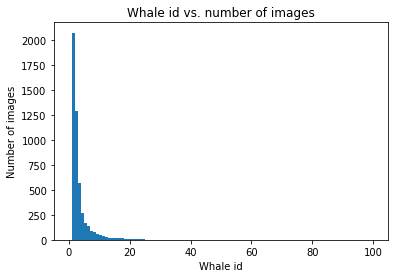
\includegraphics[width=.6\textwidth]{images/whale_frequency.png}
	\caption{\label{fig:whalefreq}: Number of images per whale}
\end{figure}

It is obvious that the problem is an instance of image classification with a large number of classes, however, when we took a look at the dataset, we discovered that there were large class imbalances in the dataset. For the remainder of this report when talking about ``classes'' we refer to individual whales. There were over 9,000 instances of unknown whales, and only 73 instances of the most frequent known whale. Table \ref{tab:counts} shows the value counts of the first few most common whales in the training set. Here we see our first problem. The \textit{new\_whale} class is vastly over-represented. Figure \ref{fig:whalefreq} shows our second problem. The value counts of the whale classes falls off exponentially. In particular, more than \textit{half} the classes have less than 5 examples, and for over 2,000 identified whales there is only one example image. This was a challenge we had to overcome with data augmentation, as described in later sections.\\

% \captionsetup[subfigure]{justification=raggedright}

\begin{figure}[h!]
	\begin{subfigure}{.5\textwidth}
		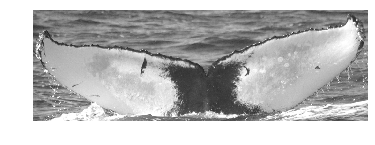
\includegraphics[width=.7\textwidth]{images/w_d3b46e7.png}
		\caption{Whale w\_d3b46e7}
	\end{subfigure}
	\begin{subfigure}{.5\textwidth}
		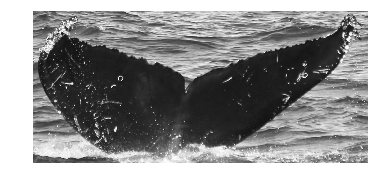
\includegraphics[width=.7\textwidth]{images/w_581ba42.png}
		\caption{Whale w\_581ba42}
	\end{subfigure}
	\begin{subfigure}{.5\textwidth}
		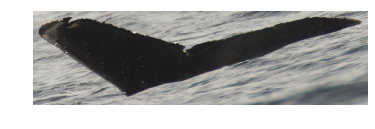
\includegraphics[width=.7\textwidth]{images/new_whale.png}
		\caption{Unidentified Whale}
	\end{subfigure}
	\begin{subfigure}{.5\textwidth}
		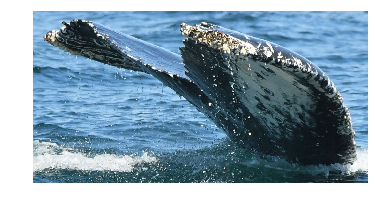
\includegraphics[width=.7\textwidth]{images/w_dd944b7.png}
		\caption{Whale w\_dd944b7}
	\end{subfigure}
	\caption{\label{fig:whale}Variety in data}
\end{figure}

There were also some challenges that had to do with the images themselves, namely, they were not of uniform size, nor were they all color or grayscale. It is quite a heterogeneous dataset. Figure \ref{fig:whale} shows four examples of images whose widths have been made uniform for display purposes. In reality, they all have very different dimensions, and some have fewer channels than others.\\
